\documentclass[12pt, letterpaper]{article}
\usepackage[utf8]{inputenc}
\usepackage{graphicx}
\usepackage{amsmath}
\title{Stochastic Layers}
\date{}

\begin{document}
\vspace{-5cm}
\maketitle
\vspace{-2cm}

\section{Architecture}
We categorize the stochastic layers based on their architecture.
Any trainable network or a layer with trainable parameters can act as a stochastic layer. 
These include (but are not limited to) convolutional layers, fully connected layers, support vector machines, recurrent networks like LSTMs, transformers, etc. In this section we discuss convolutional stochastic layers and fully connected stochastic layers as physical incarnations of the stochastic layers.  
\begin{figure}[h!]
    \centering
    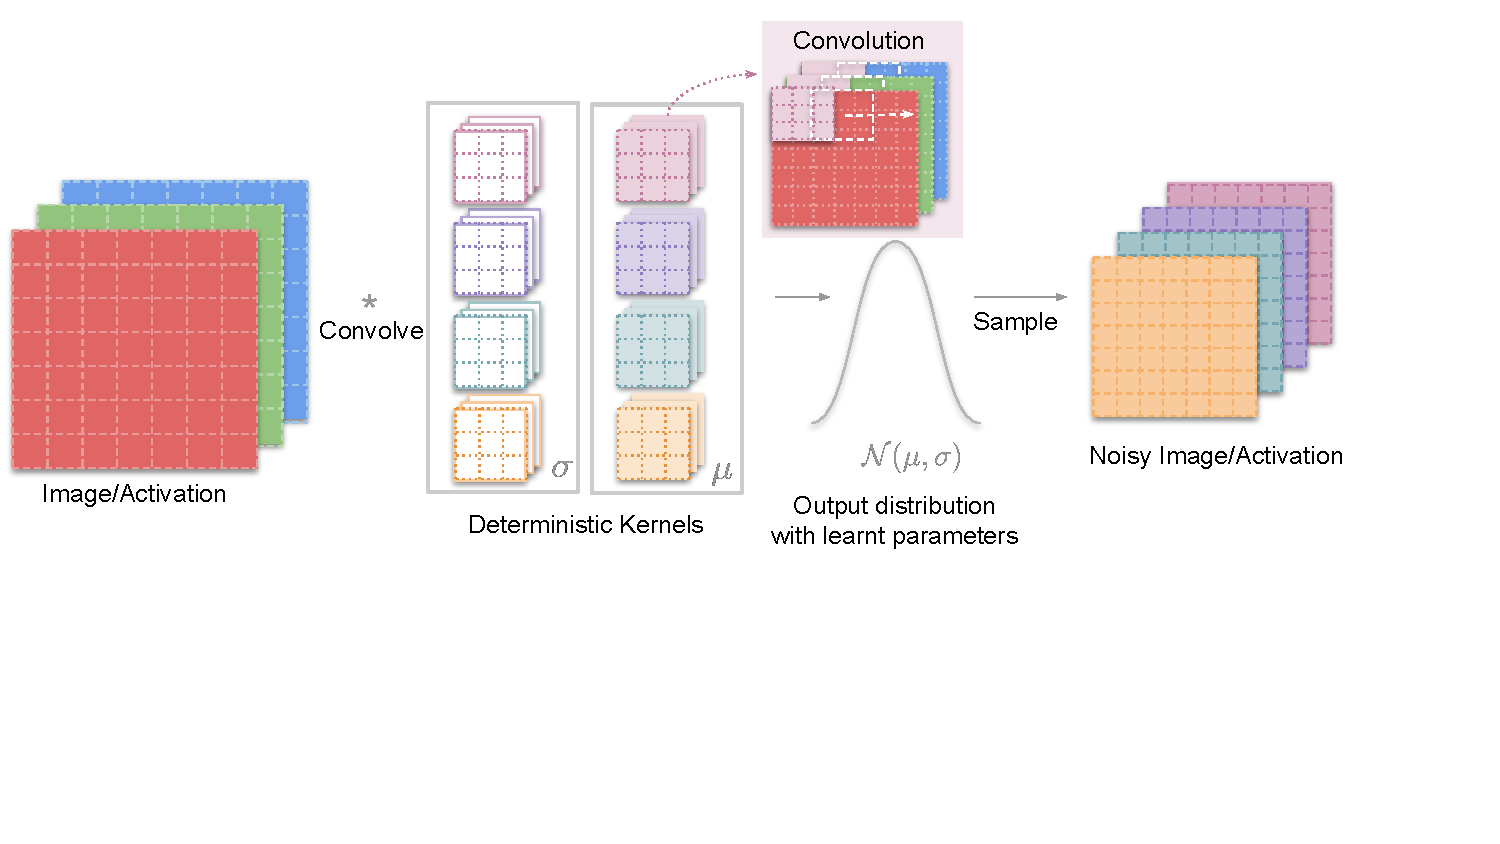
\includegraphics[width=\textwidth, trim={0 5cm 2.5cm 0}, clip]{deterministic(1).pdf}
    \caption{Stochastic layer with deterministic convolutional kernels.}
    \label{fig:deterministic}
\end{figure}

\subsection{Convolutional Stochastic layer}
\label{sec:conv}
Convolution (in the context of neural networks) is a linear mathematical operation where a kernel $k$ slides across an input tensor $x$ performing a linear operation at every location of the tensor, thereby transforming the tensor in a certain way. 
The output of this operation is a tensor $h_k$ which represents a feature (also called an activation). 
In a convolutional layer of a neural network, the input tensor $x$ is passed through a number of kernels, whose parameters are learnt during training through backpropagation. 
The activations $h_k$ from the respective kernels $k$ are stacked into channels to form the output $h=[h_k]$. Eq.~\eqref{eq:conv} shows the convolution operation. 
In Eq.~\eqref{eq:conv}, $[m,n]$ represents the spatial coordinates of the output tensor $h_k$, $[i,j]$ represents the spatial coordinates of the kernel $k$.
\begin{equation}
  h_k[m,n]=(x * k)[m,n]=\sum_i \sum_j k[i,j]x[m+i,n+j]
  \label{eq:conv}
\end{equation}

We have the following two proposed mechanisms for learning the kernels in the convolutional stochastic layers.

\begin{figure}[h!]
    \centering
    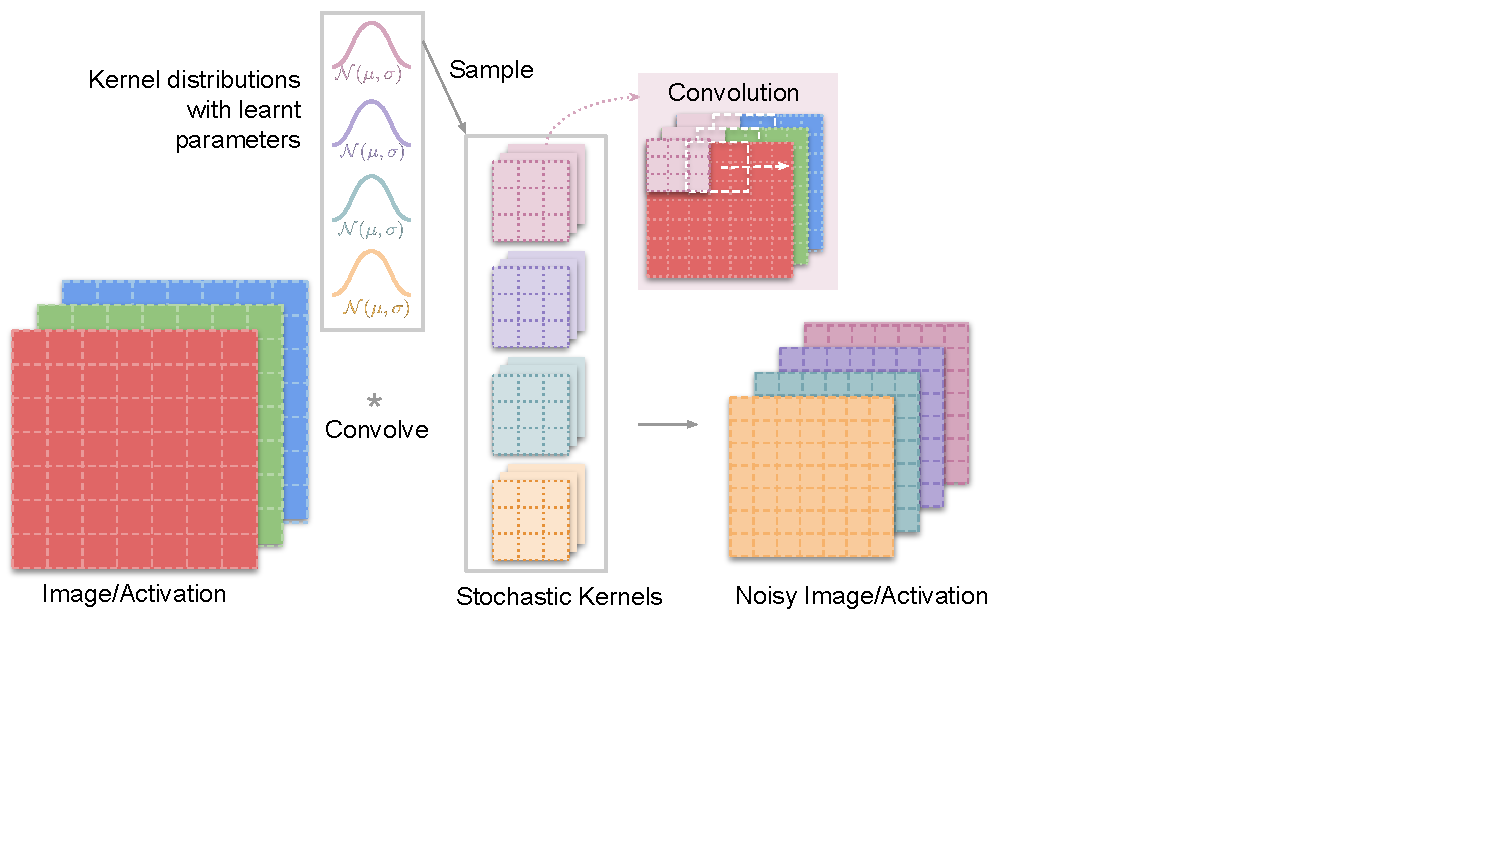
\includegraphics[width=\textwidth, trim={0 3cm 8.5cm 0}, clip]{stochastic(1).pdf}
    \caption{Stochastic layer with stochastic convolutional kernels.}
    \label{fig:stochastic}
\end{figure}
\subsubsection{Deterministic Kernels for Convolutional Stochastic Layers}
The deterministic kernels are used to produce outputs which act as parameters of a probability distribution. 
Any probability distribution is applicable according to the use case including (but not limited to) gaussian, binomial and multinomial distributions.  
Fig.~\ref{fig:deterministic} shows the mechanism where the kernels convolve over an input to produce the parameters of a gaussian distribution. 
Next, we elaborate the forward pass, training procedure and inference by assuming a gaussian distribution for the output activations.

\textbf{Forward Pass}: Prior to training, two sets of kernels ($k_\mu$ and $k_\sigma$) are initialized for the two parameters in a gaussian distrubution $\mu$ and $\sigma$ respectively. During the forward pass, the kernels $k_\mu$ and $k_\sigma$ perform convolution operation on the input activation $x$. The output activation maps ($\mu$ and $\sigma$) are obtained from the respective set of kernels according to Eq.~\eqref{eq:mu} and Eq.~\eqref{eq:sigma}. $\mu$ and $\sigma$ are used to define the gaussian distribution. We randomly sample an activation map  $h_\mathrm{sample}$ from this distribution according to Eq.~\eqref{eq:sample}. $h_\mathrm{sample}$ acts as an input activation for the next layers in the network. 

\begin{equation}
  \mu[m,n]=(x * k_\mu)[m,n]=\sum_i \sum_j k_\mu[i,j]x[m+i,n+j]
  \label{eq:mu}
\end{equation}
\begin{equation}
  \sigma[m,n]=(x * k_\sigma)[m,n]=\sum_i \sum_j k_\sigma[i,j]x[m+i,n+j]
  \label{eq:sigma}
\end{equation}

\begin{align}
  h_\mathrm{sample} \sim \mathcal{N}(\mu,\sigma) \notag\\
  \Rightarrow h_\mathrm{sample}=\mu + \sigma.\epsilon;\; \epsilon \sim \mathcal{N}(0,1)
  \label{eq:sample}
\end{align}

\textbf{Training}: The deterministic kernels are trained in a similar manner as standard convolutional neural networks. The parameters of the gaussian distribution $\mu$ and $\sigma$ (Eq.~\eqref{eq:mu} and Eq.~\eqref{eq:sigma}), obtained in the forward pass, are differentiable with respect to the kernels $k_\mu$ and $k_\sigma$ respectively. $h_\mathrm{sample}$ is differentiable with respect to $\mu$ and $\sigma$. Gradients of the output activation $h_\mathrm{sample}$ can be obtained with respect to the kernels  $k_\mu$ and $k_\sigma$. The kernels are trainable using the aforementioned gradients through back-propagation and gradient descent. 

\textbf{Inference}:
The kernels $k_\mu$ and $k_\sigma$ are trained according to the previous sub-section. A forward pass is performed using the trained kernels to produce the output activation map $h_\mathrm{sample}$. The output activation map acts as an input activation for the next layer in the neural network. %trained kernels $k_\mu$ and $k_\sigma$ convolve with an input activation $x$ and produce the parameters $\mu$ and $\sigma$ of a gaussian distribution (Eq.~\eqref{eq:mu} and Eq.~\eqref{eq:conv}). The output $h_\mathrm{sample}$ is drawn from $\mathcal{N}(\mu, \sigma)$ according to Eq.~\eqref{eq:sample}. $h_\mathrm{sample}$ acts as an input activation for the next layer in the neural network.

\subsubsection{Stochastic Kernels for Convolutional Stochastic Layers} 
In contrast to single-valued kernels used in standard deep networks, we can introduce stochasticity by learning a probability distribution representing each kernel. The stochastic kernels are drawn from the respective probability distributions, according to Eq.~\eqref{eq:sample_kernel}. The parameters of the probability distributions are trainable. 
Any probability distribution is applicable for a kernel according to the use case including (but not limited to) gaussian, binomial and multinomial distributions.  
Fig.~\ref{fig:stochastic} shows the mechanism where the kernels, sampled from respective gaussian distributions,  convolve over an input to produce an output activation map. 
Next, we elaborate the forward pass, training procedure and inference by assuming gaussian distributions for the kernels. 

\textbf{Forward Pass}: Prior to training, the parameters ($\mu_{k_\mathrm{stoc.}}$, $\sigma_{k_\mathrm{stoc.}}$), representing a gaussian for each kernel distribution, are initialized. During forward pass, a kernel $k_\mathrm{stoc.}$ is drawn from each distribution according to Eq.~\eqref{eq:sample_kernel}. $k_\mathrm{stoc.}$ convolves over the input activation $x$ to produce the output activation ($h_{k_\mathrm{stoc.}}$) (Eq.~\eqref{eq:stoc.}).

\begin{equation}
  h_{k_\mathrm{stoc.}}[m,n]=(x * k_\mathrm{stoc.})[m,n]=\sum_i \sum_j k_\mathrm{stoc.}[i,j]x[m+i,n+j]
  \label{eq:stoc.}
\end{equation}
 
\begin{align}
  k_\mathrm{stoc.} \sim \mathcal{N}(\mu_{k_\mathrm{stoc.}},\sigma_{k_\mathrm{stoc.}}) \notag\\
  \Rightarrow k_\mathrm{stoc.}=\mu_{k_\mathrm{stoc.}} + \sigma_{k_\mathrm{stoc.}}.\epsilon;\; \epsilon \sim \mathcal{N}(0,1)
  \label{eq:sample_kernel}
\end{align}

\textbf{Training}: The parameters of the gaussian distribution ($\mu_{k_\mathrm{stoc.}}$, $\sigma_{k_\mathrm{stoc.}}$) for each kernel $k$ are trainable. The output activation $h_{k_\mathrm{stoc.}}$ is differentiable with respect to the kernels $k_\mathrm{stoc.}$. The kernels $k_\mathrm{stoc.}$ are differentiable with respect to parameters ($\mu_{k_\mathrm{stoc.}}$, $\sigma_{k_\mathrm{stoc.}}$). Gradients of the output activation $h_{k_\mathrm{stoc.}}$ can be obtained with respect to the parameters ($\mu_{k_\mathrm{stoc.}}$, $\sigma_{k_\mathrm{stoc.}}$). Back-propagation and gradient descent are directly applicable. 

\textbf{Inference}:
The parameters ($\mu_{k_\mathrm{stoc.}}$, $\sigma_{k_\mathrm{stoc.}}$), representing each kernel distribution, are trained following the previous sub-section.
A forward pass is performed using the trained parameters to produce the output activation map $h_{k_\mathrm{stoc.}}$%kernel $k_\mathrm{stoc.}$ is drawn from the respective distributions with trained parameters. $k_\mathrm{stoc.}$ convolves over the input activation $x$. The output activation map ($h_{k_\mathrm{stoc.}}$) is obtained from the respective kernels according to Eq.~\eqref{eq:stoc.}.
which acts as an input activation for the next layer in the neural network.

\subsection{Fully Connected Stochastic Layer}
A fully connected layer performs the inner-product between the input activation vector ($x$) and the trainable parameter vector $W$.
This is represented by Eq.~\eqref{eq:linear}. The vector $h$ represents the output activation that propagates forward.
\begin{equation}
h=W \cdot x
    \label{eq:linear}
\end{equation}

\subsubsection{Deterministic Weight Vector for Fully Connected Stochastic Layers} 
The deterministic weight vectors are used to produce output activations which act as parameters of a probability distribution. 
Any probability distribution is applicable according to the use case including (but not limited to) gaussian, binomial and multinomial distributions.  
We discuss the forward pass, training and inference procedure, by assuming a gaussian probability distribution for the output activation. 

\textbf{Forward Pass}: Prior to training, two sets of weight vectors ($W_\mu$ and $W_\sigma$) are initialized for the two parameters $\mu$ and $\sigma$. During each forward pass, inner product between the input activation $x$ and the weight vectors $W_\mu$ and $W_\sigma$ produces the output activation maps $\mu$ and $\sigma$ according to Eq.~\eqref{eq:mu_inn} and Eq.~\eqref{eq:sigma_inn}. $\mu$ and $\sigma$ are used to define the gaussian distribution. We randomly sample an activation map  $h_\mathrm{sample}$ from this distribution according to Eq.~\eqref{eq:sample_inn}. $h_\mathrm{sample}$ acts as an input activation for the following layers in the network. 

\begin{equation}
\mu=W_\mu \cdot x
\label{eq:mu_inn}
\end{equation}

\begin{equation}
\sigma=W_\sigma \cdot x
\label{eq:sigma_inn}
\end{equation}

\begin{align}
  h_\mathrm{sample} \sim \mathcal{N}(\mu,\sigma) \notag\\
  \Rightarrow h_\mathrm{sample}=\mu + \sigma.\epsilon;\; \epsilon \sim \mathcal{N}(0,1)
  \label{eq:sample_inn}
\end{align}


\textbf{Training}: The deterministic weight vectors are trained in a similar manner as standard fully connected layers in a neural networks. The parameters of the gaussian distribution $\mu$ and $\sigma$ (Eq.~\eqref{eq:mu_inn} and Eq.~\eqref{eq:sigma_inn}), from the forward pass, are differentiable with respect to the weight vectors $W_\mu$ and $W_\sigma$ respectively. $h_\mathrm{sample}$ is differentiable with respect to $\mu$ and $\sigma$. Gradients of the output activation $h_\mathrm{sample}$ can be obtained with respect to $W_\mu$ and $W_\sigma$. The weights are trainable using back-propagation and gradient descent. 

\textbf{Inference}:
The weight vectors $W_\mu$ and $W_\sigma$ are trained according to the previous sub-section. A forward pass is performed using the trained weight vectors to produce the output activation map $h_\mathrm{sample}$. The output activation map acts as an input activation for the next layer in the neural network.

\subsubsection{Stochastic Weight Vector for Fully Connected Stochastic Layers} 

In contrast to single-valued weight vectors used in standard deep networks, we can introduce stochasticity by learning a probability distribution representing the weights. The stochastic weight vectors are drawn from the learnt probability distribution, according to Eq.~\eqref{eq:sample_weight}. The parameters of the probability distribution are trainable. 
Any probability distribution is applicable according to the use case including (but not limited to) gaussian, binomial and multinomial distributions.  
Next, we discuss the forward pass, training procedure and inference by assuming the trainable probability distribution for the weight vector to be a gaussian. 

\textbf{Forward Pass}: Prior to training, the parameters ($\mu_{W_\mathrm{stoc.}}$, $\sigma_{W_\mathrm{stoc.}}$) representing a gaussian are initialized. During forward pass, a weight vector is sampled from each distribution according to Eq.~\eqref{eq:sample_weight}. Inner product of the input activation $x$ and $W_\mathrm{stoc.}$ produces the output activation ($h_{W_\mathrm{stoc.}}$) according to Eq.~\eqref{eq:stoc_inn}.

\begin{equation}
h_{W_\mathrm{stoc.}}=W_\mathrm{stoc.} \cdot x
\label{eq:stoc_inn}
\end{equation}
 
\begin{align}
  W_\mathrm{stoc.} \sim \mathcal{N}(\mu_{W_\mathrm{stoc.}},\sigma_{W_\mathrm{stoc.}}) \notag\\
  \Rightarrow W_\mathrm{stoc.}=\mu_{W_\mathrm{stoc.}} + \sigma_{W_\mathrm{stoc.}}.\epsilon;\; \epsilon \sim \mathcal{N}(0,1)
  \label{eq:sample_weight}
\end{align}

\textbf{Training}: The parameters of the gaussian distribution ($\mu_{W_\mathrm{stoc.}}$, $\sigma_{W_\mathrm{stoc.}}$) are trainable. The output activation $h_{W_\mathrm{stoc.}}$ is differentiable with respect to $W_\mathrm{stoc.}$. The weight vector $W_\mathrm{stoc.}$ is differentiable with respect to parameters ($\mu_{W_\mathrm{stoc.}}$, $\sigma_{W_\mathrm{stoc.}}$). Gradients of the output activation $h_{W_\mathrm{stoc.}}$ can be obtained with respect to ($\mu_{W_\mathrm{stoc.}}$, $\sigma_{W_\mathrm{stoc.}}$). Back-propagation and gradient descent are directly applicable. 

\textbf{Inference}:
The parameters ($\mu_{W_\mathrm{stoc.}}$, $\sigma_{W_\mathrm{stoc.}}$), representing a distribution for the weight vector, are trained following the previous sub-section.
A forward pass is performed using the trained parameters to produce the output activation map $h_{W_\mathrm{stoc.}}$ which acts as an input activation for the next layer in the neural network.


\section{Embodiments of Stochastic Layers}
We consider a neural network $N$, input $x$, a stochastic layer $S_L$, and $n$ additional regular layers $L_{i\text{\{$i=0$ to $n$\}}}$. In the normal state of using $N$, the input is applied to $N$ without the involvement of $S_L$ or $L_i$. We propose a few embodiments as described below.
\begin{enumerate}
    \item In one embodiment, we propose this new arrangement as shown. $x \rightarrow L_{i\text{\{$i=0$ to $n$\}}} \rightarrow S_L \rightarrow N$.
    \item In another embodiment, we break $N$ into two parts $N_1$ and $N_2$, where $N$ is equivalent to $N_1$,$N_2$ back to back. Let $O_1$ be the output of applying $N_1$ to $x$, i.e., $O_1 = x \rightarrow N_1$. Let $O_2$ be the output of applying $L_{i\text{\{$i=0$ to $n$\}}}$ to $x$, i.e., $O_2 = x \rightarrow L_{i\text{\{$i=0$ to $n$\}}}$. Then, we merge $O_1$ and $O_2$ and pass the merged results through $S_L$. We then pass the resulting activations through $N_2$.
    \item In another embodiment, we apply $S_L$ to $O_2$, then merge the results with $O_1$, and then pass the result through $N_2$.
    
\end{enumerate}

\end{document}
